\documentclass{standalone}
\usepackage{tikz}
\usetikzlibrary{patterns}
\usetikzlibrary{positioning}
\usetikzlibrary{patterns, positioning}
\usetikzlibrary{shapes.misc}
\usepackage[outline]{contour}
\contourlength{1.5pt} 
\usepackage[sfdefault]{ClearSans}

\begin{document}
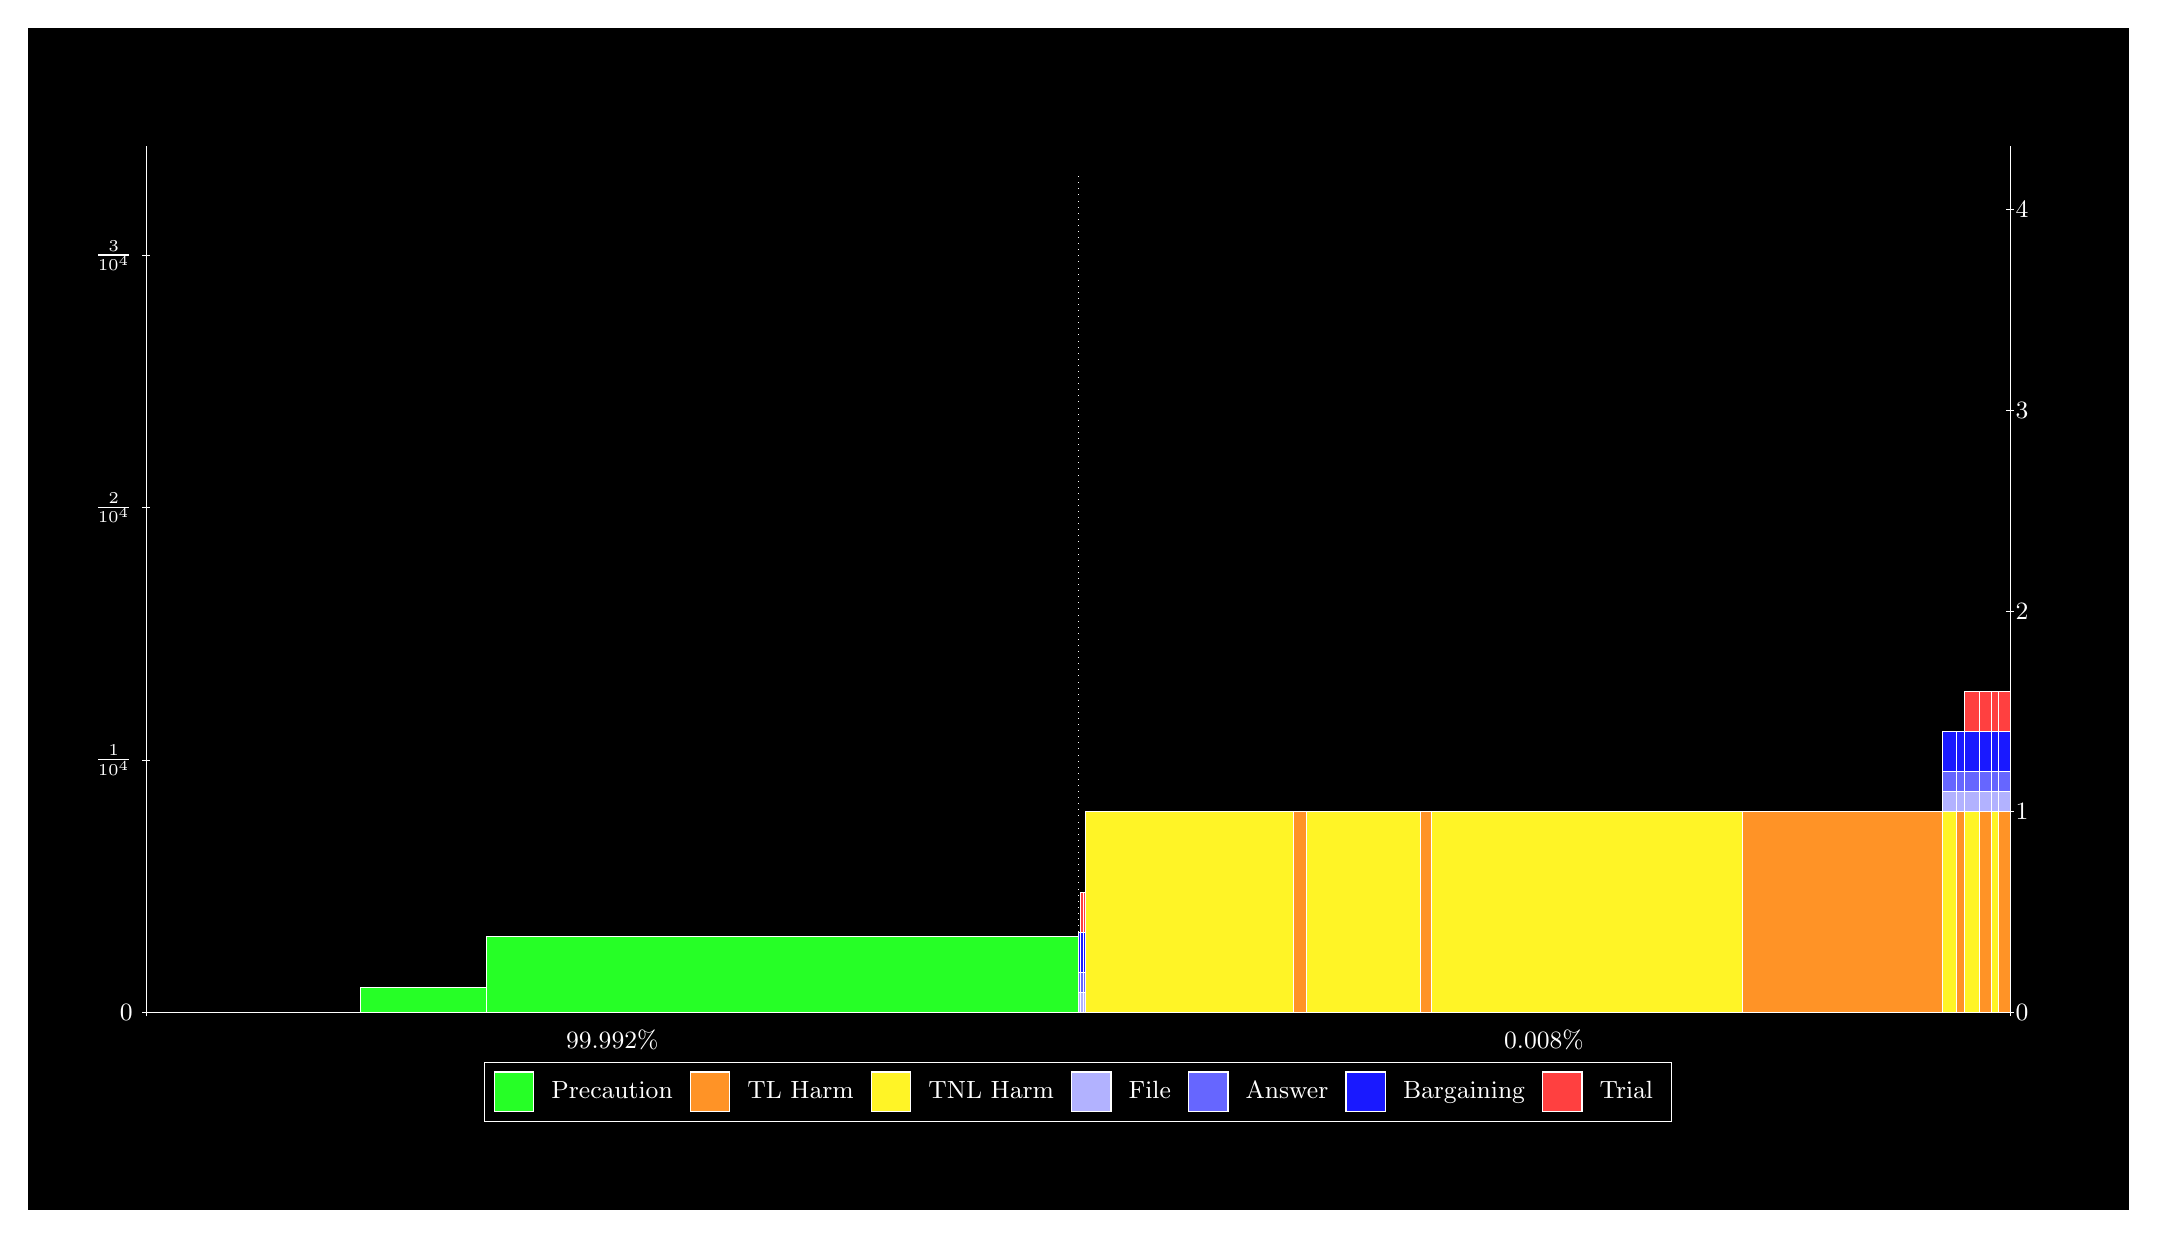
\begin{tikzpicture}
\draw[fill=black] (0,0) rectangle (26.667,15);
\draw[fill=green!85,draw=white,very thin] (4.2218,2.5) rectangle (5.8205,2.8205);
\draw[fill=green!85,draw=white,very thin] (5.8205,2.5) rectangle (13.333,3.4616);
\draw[fill=blue!30,draw=white,very thin] (13.333,2.5) rectangle (13.361,2.7549);
\draw[fill=blue!60,draw=white,very thin] (13.333,2.7549) rectangle (13.361,3.0098);
\draw[fill=blue!90,draw=white,very thin] (13.333,3.0098) rectangle (13.361,3.5197);
\draw[fill=blue!30,draw=white,very thin] (13.361,2.5) rectangle (13.395,2.7549);
\draw[fill=blue!60,draw=white,very thin] (13.361,2.7549) rectangle (13.395,3.0098);
\draw[fill=blue!90,draw=white,very thin] (13.361,3.0098) rectangle (13.395,3.5197);
\draw[fill=red!75,draw=white,very thin] (13.361,3.5197) rectangle (13.395,4.0295);
\draw[fill=green!85,draw=white,very thin] (13.395,2.5) rectangle (13.422,2.5);
\draw[fill=blue!30,draw=white,very thin] (13.395,2.5) rectangle (13.422,2.7549);
\draw[fill=blue!60,draw=white,very thin] (13.395,2.7549) rectangle (13.422,3.0099);
\draw[fill=blue!90,draw=white,very thin] (13.395,3.0099) rectangle (13.422,3.5197);
\draw[fill=red!75,draw=white,very thin] (13.395,3.5197) rectangle (13.422,4.0295);
\draw[fill=yellow!85,draw=white,very thin] (13.422,2.5) rectangle (16.06,5.0491);
\draw[fill=orange!85,draw=white,very thin] (16.06,2.5) rectangle (16.226,5.0491);
\draw[fill=green!85,draw=white,very thin] (16.226,2.5) rectangle (17.674,2.5);
\draw[fill=yellow!85,draw=white,very thin] (16.226,2.5) rectangle (17.674,5.0492);
\draw[fill=green!85,draw=white,very thin] (17.674,2.5) rectangle (17.823,2.5);
\draw[fill=orange!85,draw=white,very thin] (17.674,2.5) rectangle (17.823,5.0492);
\draw[fill=green!85,draw=white,very thin] (17.823,2.5) rectangle (21.767,2.5001);
\draw[fill=yellow!85,draw=white,very thin] (17.823,2.5001) rectangle (21.767,5.0492);
\draw[fill=green!85,draw=white,very thin] (21.767,2.5) rectangle (24.309,2.5001);
\draw[fill=orange!85,draw=white,very thin] (21.767,2.5001) rectangle (24.309,5.0492);
\draw[fill=yellow!85,draw=white,very thin] (24.309,2.5) rectangle (24.486,5.0491);
\draw[fill=blue!30,draw=white,very thin] (24.309,5.0491) rectangle (24.486,5.3041);
\draw[fill=blue!60,draw=white,very thin] (24.309,5.3041) rectangle (24.486,5.559);
\draw[fill=blue!90,draw=white,very thin] (24.309,5.559) rectangle (24.486,6.0688);
\draw[fill=orange!85,draw=white,very thin] (24.486,2.5) rectangle (24.584,5.0491);
\draw[fill=blue!30,draw=white,very thin] (24.486,5.0491) rectangle (24.584,5.3041);
\draw[fill=blue!60,draw=white,very thin] (24.486,5.3041) rectangle (24.584,5.559);
\draw[fill=blue!90,draw=white,very thin] (24.486,5.559) rectangle (24.584,6.0688);
\draw[fill=yellow!85,draw=white,very thin] (24.584,2.5) rectangle (24.782,5.0491);
\draw[fill=blue!30,draw=white,very thin] (24.584,5.0491) rectangle (24.782,5.3041);
\draw[fill=blue!60,draw=white,very thin] (24.584,5.3041) rectangle (24.782,5.559);
\draw[fill=blue!90,draw=white,very thin] (24.584,5.559) rectangle (24.782,6.0688);
\draw[fill=red!75,draw=white,very thin] (24.584,6.0688) rectangle (24.782,6.5786);
\draw[fill=orange!85,draw=white,very thin] (24.782,2.5) rectangle (24.928,5.0491);
\draw[fill=blue!30,draw=white,very thin] (24.782,5.0491) rectangle (24.928,5.3041);
\draw[fill=blue!60,draw=white,very thin] (24.782,5.3041) rectangle (24.928,5.559);
\draw[fill=blue!90,draw=white,very thin] (24.782,5.559) rectangle (24.928,6.0688);
\draw[fill=red!75,draw=white,very thin] (24.782,6.0688) rectangle (24.928,6.5786);
\draw[fill=green!85,draw=white,very thin] (24.928,2.5) rectangle (25.022,2.5);
\draw[fill=yellow!85,draw=white,very thin] (24.928,2.5) rectangle (25.022,5.0492);
\draw[fill=blue!30,draw=white,very thin] (24.928,5.0492) rectangle (25.022,5.3041);
\draw[fill=blue!60,draw=white,very thin] (24.928,5.3041) rectangle (25.022,5.559);
\draw[fill=blue!90,draw=white,very thin] (24.928,5.559) rectangle (25.022,6.0688);
\draw[fill=red!75,draw=white,very thin] (24.928,6.0688) rectangle (25.022,6.5787);
\draw[fill=green!85,draw=white,very thin] (25.022,2.5) rectangle (25.167,2.5);
\draw[fill=orange!85,draw=white,very thin] (25.022,2.5) rectangle (25.167,5.0492);
\draw[fill=blue!30,draw=white,very thin] (25.022,5.0492) rectangle (25.167,5.3041);
\draw[fill=blue!60,draw=white,very thin] (25.022,5.3041) rectangle (25.167,5.559);
\draw[fill=blue!90,draw=white,very thin] (25.022,5.559) rectangle (25.167,6.0688);
\draw[fill=red!75,draw=white,very thin] (25.022,6.0688) rectangle (25.167,6.5787);
\draw[white,very thin] (1.5,2.5) -- (1.5,13.5);
\draw[white,very thin] (1.45,2.5) -- (1.55,2.5);
\node[font=\small,text=white, anchor=east] at (1.45, 2.5) {0};
\draw[white,very thin] (1.45,5.7052) -- (1.55,5.7052);
\node[font=\small,text=white, anchor=east] at (1.45, 5.7052) {$\frac{1}{10^{4}}$};
\draw[white,very thin] (1.45,8.9104) -- (1.55,8.9104);
\node[font=\small,text=white, anchor=east] at (1.45, 8.9104) {$\frac{2}{10^{4}}$};
\draw[white,very thin] (1.45,12.116) -- (1.55,12.116);
\node[font=\small,text=white, anchor=east] at (1.45, 12.116) {$\frac{3}{10^{4}}$};

\draw[white,dotted,very thin] (13.333,2.83) -- (13.333,13.17);
\draw[white,very thin] (25.167,2.5) -- (25.167,13.5);
\draw[white,very thin] (25.117,2.5) -- (25.217,2.5);
\node[font=\small,text=white, anchor=west] at (25.117, 2.5) {0};
\draw[white,very thin] (25.117,5.0491) -- (25.217,5.0491);
\node[font=\small,text=white, anchor=west] at (25.117, 5.0491) {1};
\draw[white,very thin] (25.117,7.5983) -- (25.217,7.5983);
\node[font=\small,text=white, anchor=west] at (25.117, 7.5983) {2};
\draw[white,very thin] (25.117,10.147) -- (25.217,10.147);
\node[font=\small,text=white, anchor=west] at (25.117, 10.147) {3};
\draw[white,very thin] (25.117,12.697) -- (25.217,12.697);
\node[font=\small,text=white, anchor=west] at (25.117, 12.697) {4};

\draw[white,very thin] (1.5,2.5) -- (25.167,2.5);
\draw[white,very thin] (1.5,2.45) -- (1.5,2.55);
\node[font=\small,text=white, anchor=north] at (1.5, 2.45) {};
\draw[white,very thin] (25.167,2.45) -- (25.167,2.55);
\node[font=\small,text=white, anchor=north] at (25.167, 2.45) {};

\node[font=\small,text=white,anchor=south] at (7.4167, 1.9) {99.992\%};
\node[font=\small,text=white,anchor=south] at (19.25, 1.9) {0.008\%};
\draw (13.3333,2.5) node (B) {};
\begin{scope}[align=center]
\matrix[scale=0.5,draw=white,below=0.5cm of B,nodes={draw},column sep=0.1cm]{
\node[rectangle,draw,minimum width=0.5cm,minimum height=0.5cm,fill=green!85]{}; & \node[draw=none,font=\small,text=white]{Precaution}; &
\node[rectangle,draw,minimum width=0.5cm,minimum height=0.5cm,fill=orange!85]{}; & \node[draw=none,font=\small,text=white]{TL Harm}; &
\node[rectangle,draw,minimum width=0.5cm,minimum height=0.5cm,fill=yellow!85]{}; & \node[draw=none,font=\small,text=white]{TNL Harm}; &
\node[rectangle,draw,minimum width=0.5cm,minimum height=0.5cm,fill=blue!30]{}; & \node[draw=none,font=\small,text=white]{File}; &
\node[rectangle,draw,minimum width=0.5cm,minimum height=0.5cm,fill=blue!60]{}; & \node[draw=none,font=\small,text=white]{Answer}; &
\node[rectangle,draw,minimum width=0.5cm,minimum height=0.5cm,fill=blue!90]{}; & \node[draw=none,font=\small,text=white]{Bargaining}; &
\node[rectangle,draw,minimum width=0.5cm,minimum height=0.5cm,fill=red!75]{}; & \node[draw=none,font=\small,text=white]{Trial}; \\\\
};\end{scope}

\end{tikzpicture}
\end{document}